\documentclass[border=4pt]{standalone}
% Shared typography and colours for the standalone figures.
\usepackage{unicode-math}
\setmainfont{TeX Gyre Termes}
\setmathfont{TeX Gyre Termes Math}
\usepackage{tikz}
\usetikzlibrary{arrows.meta,positioning,calc,decorations.pathreplacing}
\usepackage{pgfplots}
\pgfplotsset{compat=1.18}

% One colour per element or subsystem. Record the mapping in
% the working repository conventions and use it identically in every figure.
\definecolor{elemA}{HTML}{1F5FA8}
\definecolor{elemB}{HTML}{B8461B}
\definecolor{elemC}{HTML}{2E7D32}
\definecolor{elemD}{HTML}{6A4C93}
\definecolor{frameline}{HTML}{555555}

\begin{document}
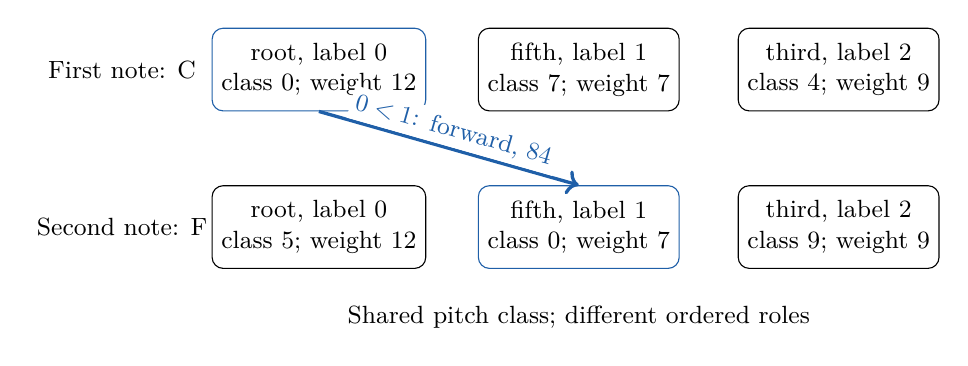
\begin{tikzpicture}[font=\small,box/.style={draw,rounded corners,minimum width=2.5cm,minimum height=1.05cm,align=center}]
\node at (-2.5,2) {First note: C};
\node at (-2.5,0) {Second note: F};
\node[box,draw=elemA] (a0) at (0,2) {root, label 0\\class 0; weight 12};
\node[box] (a1) at (3.3,2) {fifth, label 1\\class 7; weight 7};
\node[box] (a2) at (6.6,2) {third, label 2\\class 4; weight 9};
\node[box] (b0) at (0,0) {root, label 0\\class 5; weight 12};
\node[box,draw=elemA] (b1) at (3.3,0) {fifth, label 1\\class 0; weight 7};
\node[box] (b2) at (6.6,0) {third, label 2\\class 9; weight 9};
\draw[->,very thick,elemA] (a0.south) -- node[midway,sloped,above,fill=white,inner sep=2pt] {$0<1$: forward, $84$} (b1.north);
\node[align=center] at (3.3,-1.15) {Shared pitch class; different ordered roles};
\end{tikzpicture}
\end{document}
